\documentclass[conference]{IEEEtran}
\IEEEoverridecommandlockouts

\usepackage{cite}
\usepackage{amsmath,amssymb,amsfonts}
\usepackage{algorithmic}
\usepackage{graphicx}
\usepackage{textcomp}
\usepackage{xcolor}
\usepackage{multirow}
\usepackage{booktabs}
\usepackage{algorithm}
\usepackage{algorithmic}
\def\BibTeX{{\rm B\kern-.05em{\sc i\kern-.025em b}\kern-.08em
    T\kern-.1667em\lower.7ex\hbox{E}\kern-.125emX}}
\usepackage{fontspec}
\setmainfont{Times New Roman}
\newfontfamily\cyrillicfont{Times New Roman}
\newfontfamily\mongolianfont{Times New Roman}
\usepackage{polyglossia}

\setmainlanguage{mongolian}
\setotherlanguage{english}

% we propose a novel framework called Self-Supervised Graph Neural Network (SelfGNN) - гэхээр загвар болж байна.

\begin{document}

% \title{Граф нейрал сүлжээний SelfGNN загварт суурилсан харилцагч–борлуулагчийн санал болгох систем дэх графын нэмэлт шинжүүдийн нөлөөллийн судалгаа\\}

\title{Харилцагч–борлуулагчийг санал болгох SelfGNN загварын графын шинжийн нөлөөлөл\\}

\author{\IEEEauthorblockN{Эрдэнэчимэгийн Алтаншагай}
\IEEEauthorblockA{\textit{Машин оюуны лаборатори, МКУТ, МТЭС} \\
\textit{Монгол Улсын Их Сургууль}\\
Монгол Улс, Улаанбаатар хот \\
22b1num0331@stud.num.edu.mn}
\and
\IEEEauthorblockN{Ганболдын Амарсанаа}
\IEEEauthorblockA{\textit{Машин оюуны лаборатори, МКУТ, МТЭС} \\
\textit{Монгол Улсын Их Сургууль}\\
Монгол Улс, Улаанбаатар хот \\
amarsanaag@num.edu.mn}
}

\maketitle
\renewcommand{\abstractname}{Хураангуй}
\begin{abstract}
Граф нейрон сүлжээ ашигласан санал болгох системүүд хоёр зүйлийн харилцааг голлон авч үздэг ч графын орой болон ирмэгийн  шинжүүдийн нөлөөг бага тусгасан байдаг. Энэхүү судалгаанд цаг хугацааны граф суурьтай SelfGNN загварт оройн шинж, тухайлбал, харилцагч болон борлуулагчийн шинж чанар болон ирмэгийн жинг болгож үнэлгээг нэгтгэж, борлуулагч санал болгох системийн гүйцэтгэлд үзүүлэх нөлөөг графын дөрвөн хувилбараар харьцуулан шинжилсэн. Эдгээрийг Yelp өгөгдлийн бүрдэлд туршихад оройн шинжийг дангаар нь нэгтгэсэн туршилт гүйцэтгэлийг хамгийн их сайжруулсан (HR@10: $+1.34\%$, NDCG@10: $+2.20\%$) бол ирмэгийн жин бага зэрэг ($<1\%$) сайжруулсан. Хоёр шинжийг зэрэг ашиглахад суурь загвараас доогуур гүйцэтгэл үзүүлсэн болно.
\end{abstract}

\begin{IEEEkeywords}
граф нейрон сүлжээ, санал болгох систем, SelfGNN, борлуулагч санал болгох
\end{IEEEkeywords}

\section{Танилцуулга}

Санал болгох системүүд хэрэглэгчийн зан төлөвт суурилан дараагийн боломжит зүйлийг таамаглахад чиглэсэн байдаг. Борлуулагч санал болгох нь харилцагчийн гүйлгээний түүх дээр үндэслэн харилцагчид дараа нь үйлчлэх магадлалтай боломжит борлуулагчийг олж танилцуулах зорилготой. Гэвч энэхүү асуудал нь өгөгдлийн сийрэг байдал, харилцагчийн зан төлөвийн өөрчлөлт, мөн харилцагч болон борлуулагчийн нэмэлт шинжүүдийг хэрхэн нэгтгэх зэрэг сорилтыг бий болгоно.

Сүүлийн жилүүдэд граф нейрон сүлжээнд (GNN - Graph Neural Network) суурилсан аргууд нь харилцагч–объектын харилцан үйлдлийг граф хэлбэрээр илэрхийлж, өндөр эрэмбийн хамаарлыг загварчлах боломжийг олгосон. Тэдгээрийн дотроос SelfGNN~\cite{selfgnn2024} нь цаг хугацааны мэдээллийг ашиглан дараалал болон граф бүтцийг хослуулсан үр дүнтэй загвар юм. Гэсэн хэдий ч энэхүү загвар нь зөвхөн хоёр төрөлт орой бүхий графт тулгуурладаг бөгөөд оройн болон ирмэгийн нэмэлт шинжүүдийг ашигладаггүй.

Иймээс энэхүү судалгааны зорилго нь SelfGNN загварт оройн шинж болон ирмэгийн жинг нэгтгэх нь борлуулагч санал болгох системийн гүйцэтгэлд ямар нөлөө үзүүлэхийг тодорхойлох явдал юм. Тодруулбал, нэмэлт шинжгүй суурь загвар, ирмэгийн жин, оройн шинж болон эдгээрийг бүгдийг хослуулан туршиж, тэдгээрийн тусдаа болон хамтын нөлөөг үнэлсэн.

Судалгааны гол хувь нэмрийг дараах байдлаар тодорхойлж болно.
\begin{itemize}
    \item SelfGNN загварт граф илэрхийллийг сайжруулах зорилгоор оройн шинж болон ирмэгийн жинг нэгтгэх аргыг тохируулсан.
    \item Дөрвөн туршилтаар нэмэлт шинжүүдийн нөлөөг Yelp өгөгдөл дээр харьцуулан үнэлсэн.
    \item Нэмэлт шинжүүдийн хослол нь заавал нэмэгдэхүйц биш болохыг туршилтаар харуулсан.
\end{itemize}

\section{Холбоотой ажил}

\subsection{Граф нейрон сүлжээнд суурилсан санал болгох систем}

Санал болгох системүүд уламжлалт матриц задлалын аргаас гүн нейрон сүлжээнд суурилсан загвар руу эрчимтэй шилжиж байна. Ялангуяа граф нейрон сүлжээнд суурилсан аргууд нь харилцагч–объектын харилцан үйлдлийг граф бүтэц болгон илэрхийлж, олон шатлалт хөрш мэдээллийг нэгтгэх замаар хамтын шүүлтийн өндөр эрэмбийн хамаарлыг илүү үр дүнтэй загварчлах боломжийг олгож байна \cite{gao2023survey}. Ингэснээр харилцагчийн сонирхлыг илүү нарийвчлалтай ойлгож, илүү чанартай санал гаргах боломжийг бүрдүүлдэг. 

\subsection{Дараалалд суурилсан санал болгох систем}

Дараалалд суурилсан санал болгох (sequential recommendation) систем нь харилцагчийн үйлдлийн цаг хугацааны дарааллыг буюу харилцагчийн сонирхлын цаг хугацааны өөрчлөлтийг ашиглан дараагийн хамгийн боломжит объектыг таамаглахад чиглэдэг. Орчин үеийн SASRec болон Bert4Rec зэрэг аргууд өөрийн-анхааралт (self-attention) механизмыг ашиглан урт хугацааны хамаарлыг илүү оновчтой загварчилж байна~\cite{kang2018sasrec, sun2019bert4rec}. Гэсэн хэдий ч эдгээр аргууд нь зөвхөн харилцагч бүрийн дотоод дарааллыг загварчилдаг бөгөөд богино хугацааны интервалд харилцагч хоорондын хамтын харилцааг тусгадаггүй. Үүнээс гадна, харилцагчийн богино хугацааны үйлдэл дэх чимээ шуугиан, тухайлбал, түр зуурын сонирхол, санамсаргүй харилцан үйлдлийг шүүх механизм дутмаг~\cite{selfgnn2024} байна.

\subsection{Борлуулагч санал болгох}

Борлуулагч санал болгох судалгаа харьцангуй хязгаарлагдмал бөгөөд одоогийн ажлуудыг ерөнхийд нь хоёр чиглэлд ангилж болно. Нэг чиглэл нь харилцагч–борлуулагчийн хоёр төрөлт орой бүхий графыг байгуулж, графын дүрслэлд тулгуурлан холбоос таамаглал хийх арга юм \cite{yilmaz2023link}. Нөгөө нь домэйн мэдлэгийг (domain knowledge), тухайлбал харилцагчийн хүн ам зүйн мэдээлэл болон борлуулагчийн шинж чанарыг загварт шууд нэгтгэх арга бөгөөд NMF\_CSI~\cite{yoo2023merchant} нь энэ хандлагын төлөөлөх жишээ юм. Тус загвар NeuMF бүтцэд харилцагчийн хүйс, нас болон борлуулагчийн салбар, бүс нутгийн мэдээллийг далд векторт нэгтгэн сургаснаар суурь загвараас HR@10 болон NDCG@10 үзүүлэлтүүдийг тус тус ойролцоогоор 3\% болон 5\%-иар сайжруулсан.

\subsection{Графын орой ба ирмэгийн нэмэлт шинжүүдийн нөлөө}

Графт оройн болон ирмэгийн нэмэлт шинжүүдийг нэгтгэх нь загварын гүйцэтгэлийг сайжруулдгийг олон судалгаа харуулсан. GC-MC \cite{vandenberg2018gcmc} нь хоёр хэсгийн графт ирмэгийн дохиог ашиглан MovieLens-100K дээр RMSE алдааг бууруулсан. EWS-GCN \cite{sukharev2020ewsgcn} нь банкны гүйлгээний өгөгдөл дээр ирмэгийн жинг анхаарлын механизмтай нэгтгэж GAT-ийг \cite{velickovic2018gat} давсан гүйцэтгэл үзүүлсэн. Мөн 2-SEAL-RNN \cite{shumovskaia2021bank} нь цаг хугацаанд мэдрэмтгий ирмэгийн шинжийг ашиглан гүйцэтгэлийг сайжруулсан (Хүснэгт~\ref{tab:feature_comparison}). Гэвч эдгээр нэмэлт шинжүүдийн нөлөө нь өгөгдлийн онцлог болон загварын архитектураас хамааран харилцан адилгүй байна.

\begin{table}[h]
\caption{Графын нэмэлт шинжүүдийн гүйцэтгэлд үзүүлэх нөлөөллийн харьцуулалт}
\label{tab:feature_comparison}
\centering

\renewcommand{\arraystretch}{1.3}
\setlength{\tabcolsep}{6pt}

\resizebox{\columnwidth}{!}{
\begin{tabular}{|l|l|l|l|l|}
\hline
\textbf{Загвар} & \textbf{Нэмэлт шинж} & \textbf{Өгөгдөл} & \textbf{Хэмжүүр} & \textbf{Үр дүн} \\
\hline
GC-MC \cite{vandenberg2018gcmc}
  & Ирмэгийн жин (үнэлгээ) & MovieLens-100K & RMSE & 0.905 \;(\downarrow \mathbf{0.024}) \\
\hline
GAT \cite{sukharev2020ewsgcn}
  & Оройн шинж & Банкны гүйлгээ & ROC-AUC & 0.8875 \\
\hline
2-SEAL-RNN \cite{shumovskaia2021bank}
  & Ирмэгийн шинж + анхаарал &  Банкны гүйлгээ & ROC-AUC & 0.858 \;(\uparrow \mathbf{0.212}) \\
\hline
EWS-GCN \cite{sukharev2020ewsgcn}
  & Ирмэг + орой & Банкны гүйлгээ & ROC-AUC & \textbf{0.8926} \;(\uparrow 0.004) \\
\hline
\end{tabular}
}
\end{table}
 
\subsection{SelfGNN: Өөрийгөө чиглүүлдэг граф нейрон сүлжээний загвар}

Дээрх судалгаануудыг нэгтгэн үзвэл одоогийн аргууд нь цаг хугацааны динамик, харилцагч болон санал болгох обьект хоорондын хамтын харилцаа болон графын бүтцэд суурилсан өөрийгөө хянасан сургалтыг нэгдмэл байдлаар загварчлахад хязгаарлагдмал хэвээр байна. 

SelfGNN (Self-Supervised Graph Neural Networks for Sequential Recommendation) \cite{selfgnn2024} нь энэхүү асуудлыг шийдвэрлэх зорилгоор цаг хугацааны интервалд суурилсан богино хугацааны графыг байгуулж, харилцагч хоорондын хамтын харилцааг тусгадаг. Улмаар интервалын нэгтгэл болон анхаарлын механизмаар урт хугацааны зан төлөвийг олон түвшинд загварчилж, өөрийгөө хянасан сургалтаар богино хугацааны граф дахь чимээ шуугианыг бууруулдаг. Туршилтаар энэхүү загвар нь олон өгөгдлийн олонлог дээр суурь аргуудаас давуу гүйцэтгэл үзүүлсэн (Хүснэгт~\ref{tab:selfgnn_performance}). 

\begin{table}[h]
\caption{SelfGNN загварын гүйцэтгэлийн харьцуулалт (HR@10, NDCG@10)~\cite{selfgnn2024}}
\label{tab:selfgnn_performance}
\centering

\renewcommand{\arraystretch}{1.3}
\setlength{\tabcolsep}{6pt}

\resizebox{\columnwidth}{!}{
\begin{tabular}{|l|cc|cc|cc|cc|}
\hline
\textbf{Үзүүлэлт} 
& \multicolumn{2}{c|}{\textbf{Amazon}} 
& \multicolumn{2}{c|}{\textbf{Gowalla}} 
& \multicolumn{2}{c|}{\textbf{MovieLens}} 
& \multicolumn{2}{c|}{\textbf{Yelp}} \\
\cline{2-9}
& HR@10 & NDCG@10 & HR@10 & NDCG@10 & HR@10 & NDCG@10 & HR@10 & NDCG@10 \\
\hline
Суурь загвар* 
& 0.368 & 0.230 
& 0.606 & 0.418 
& 0.237 & 0.126 
& 0.346 & 0.189 \\
\hline
SelfGNN 
& \textbf{0.391} & \textbf{0.240} 
& \textbf{0.637} & \textbf{0.437} 
& \textbf{0.239} & \textbf{0.128} 
& \textbf{0.365} & \textbf{0.201} \\
\hline
\end{tabular}
}

\vspace{2pt}
\begin{flushleft}
\footnotesize{\textit{* Суурь загвар: тухайн өгөгдөл болон үзүүлэлт бүрд хамгийн сайн гүйцэтгэл үзүүлсэн загвар}}
\end{flushleft}

\end{table}

Гэвч SelfGNN нь харилцагч ба объектын хоёр төрөлт орой бүхий графыг ашигладаг бөгөөд оройн болон ирмэгийн нэмэлт шинжүүдийг тусгадаггүй. Иймээс энэхүү судалгаа нь нэмэлт шинжүүдийг графт нэгтгэх нь борлуулагч санал болгох системийн гүйцэтгэлд үзүүлэх нөлөөг харьцуулан шинжилнэ.

\section{Судалгааны арга зүй}

Энэ хэсэгт судалгааны суурь загвар болох SelfGNN-ийн арга зүйг товч танилцуулж, графын оройн болон ирмэгийн нэмэлт шинжүүдийг нэгтгэх аргыг тодорхойлно.

\subsection{Тэмдэглэгээ ба бодлогын томьёолол}

Энэхүү судалгаанд харилцагч–борлуулагчийн харилцааг цаг хугацааны динамик граф хэлбэрээр загварчилна. харилцагчдын олонлогийг $\mathcal{U} = \{u_1, \ldots, u_I\}$, борлуулагчдын олонлогийг $\mathcal{V} = \{v_1, \ldots, v_J\}$ гэж тэмдэглэнэ.

Хугацааны муж $[t_b, t_e]$-ийг $T$ тэнцүү интервалд хувааж, тухайн $t$-р интервал дахь харилцааг зэргэлдээ матриц $\mathcal{A}_t \in \mathbb{R}^{I \times J}$-аар илэрхийлнэ. Хэрэв харилцагч $u_i$ нь борлуулагч $v_j$-тай харилцсан бол $\mathcal{A}_{t,i,j} = 1$, эсрэг тохиолдолд $0$ байна.

Үүнээс гадна дараах нэмэлт мэдээллийг ашиглана:
\begin{itemize}
    \item \textbf{харилцагчийн шинж}: $\mathbf{x}_i^{(u)} \in \mathbb{R}^{d_u}$ (жишээ нь нас, хүйс, байршил, хэрэглээний давтамж)
    \item \textbf{Борлуулагчийн шинж}: $\mathbf{x}_j^{(v)} \in \mathbb{R}^{d_v}$ (жишээ нь байршил, борлуулагчийн салбар төрөл, үйлчилгээний ангилал, дундаж үнэлгээ)
    \item \textbf{Ирмэгийн жин}: $w_{t,i,j}$ (жишээ нь гүйлгээний дүн, үнэлгээ)
\end{itemize}

Мөн дараах тэмдэглэгээг ашиглана:
\begin{itemize}
    \item $\mathbf{e}_{t,i}^{(u)} \in \mathbb{R}^{d}$ — $t$-р интервал дахь  $u_i$ харилцагчийн эмбеддинг (вектор төлөөлөл)
    \item $\mathbf{e}_{t,j}^{(v)} \in \mathbb{R}^{d}$ — $v_j$ борлуулагчийн эмбеддинг
    \item $\mathbf{f}_i^{(u)} \in \mathbb{R}^{d}$ — харилцагчийн шинжээс үүсгэсэн эмбеддинг
    \item $\mathbf{f}_j^{(v)} \in \mathbb{R}^{d}$ — борлуулагчийн шинжийн эмбеддинг
\end{itemize}

Иймээс зорилго нь дээрх мэдээллүүдийг ашиглан $(T+1)$-р интервал дахь харилцагч–борлуулагчийн харилцааг таамаглах явдал юм.

\subsection{SelfGNN загварын тойм}
 
SelfGNN~\cite{selfgnn2024} нь дараалалд суурилсан санал болгох системд зориулсан өөрийгөө хянасан граф нейрал сүлжээ бөгөөд Зураг~\ref{fig:selfgnn_arch}-д үзүүлсэн гурван үндсэн бүрдэлтэй.

\begin{figure}[t]
\centering
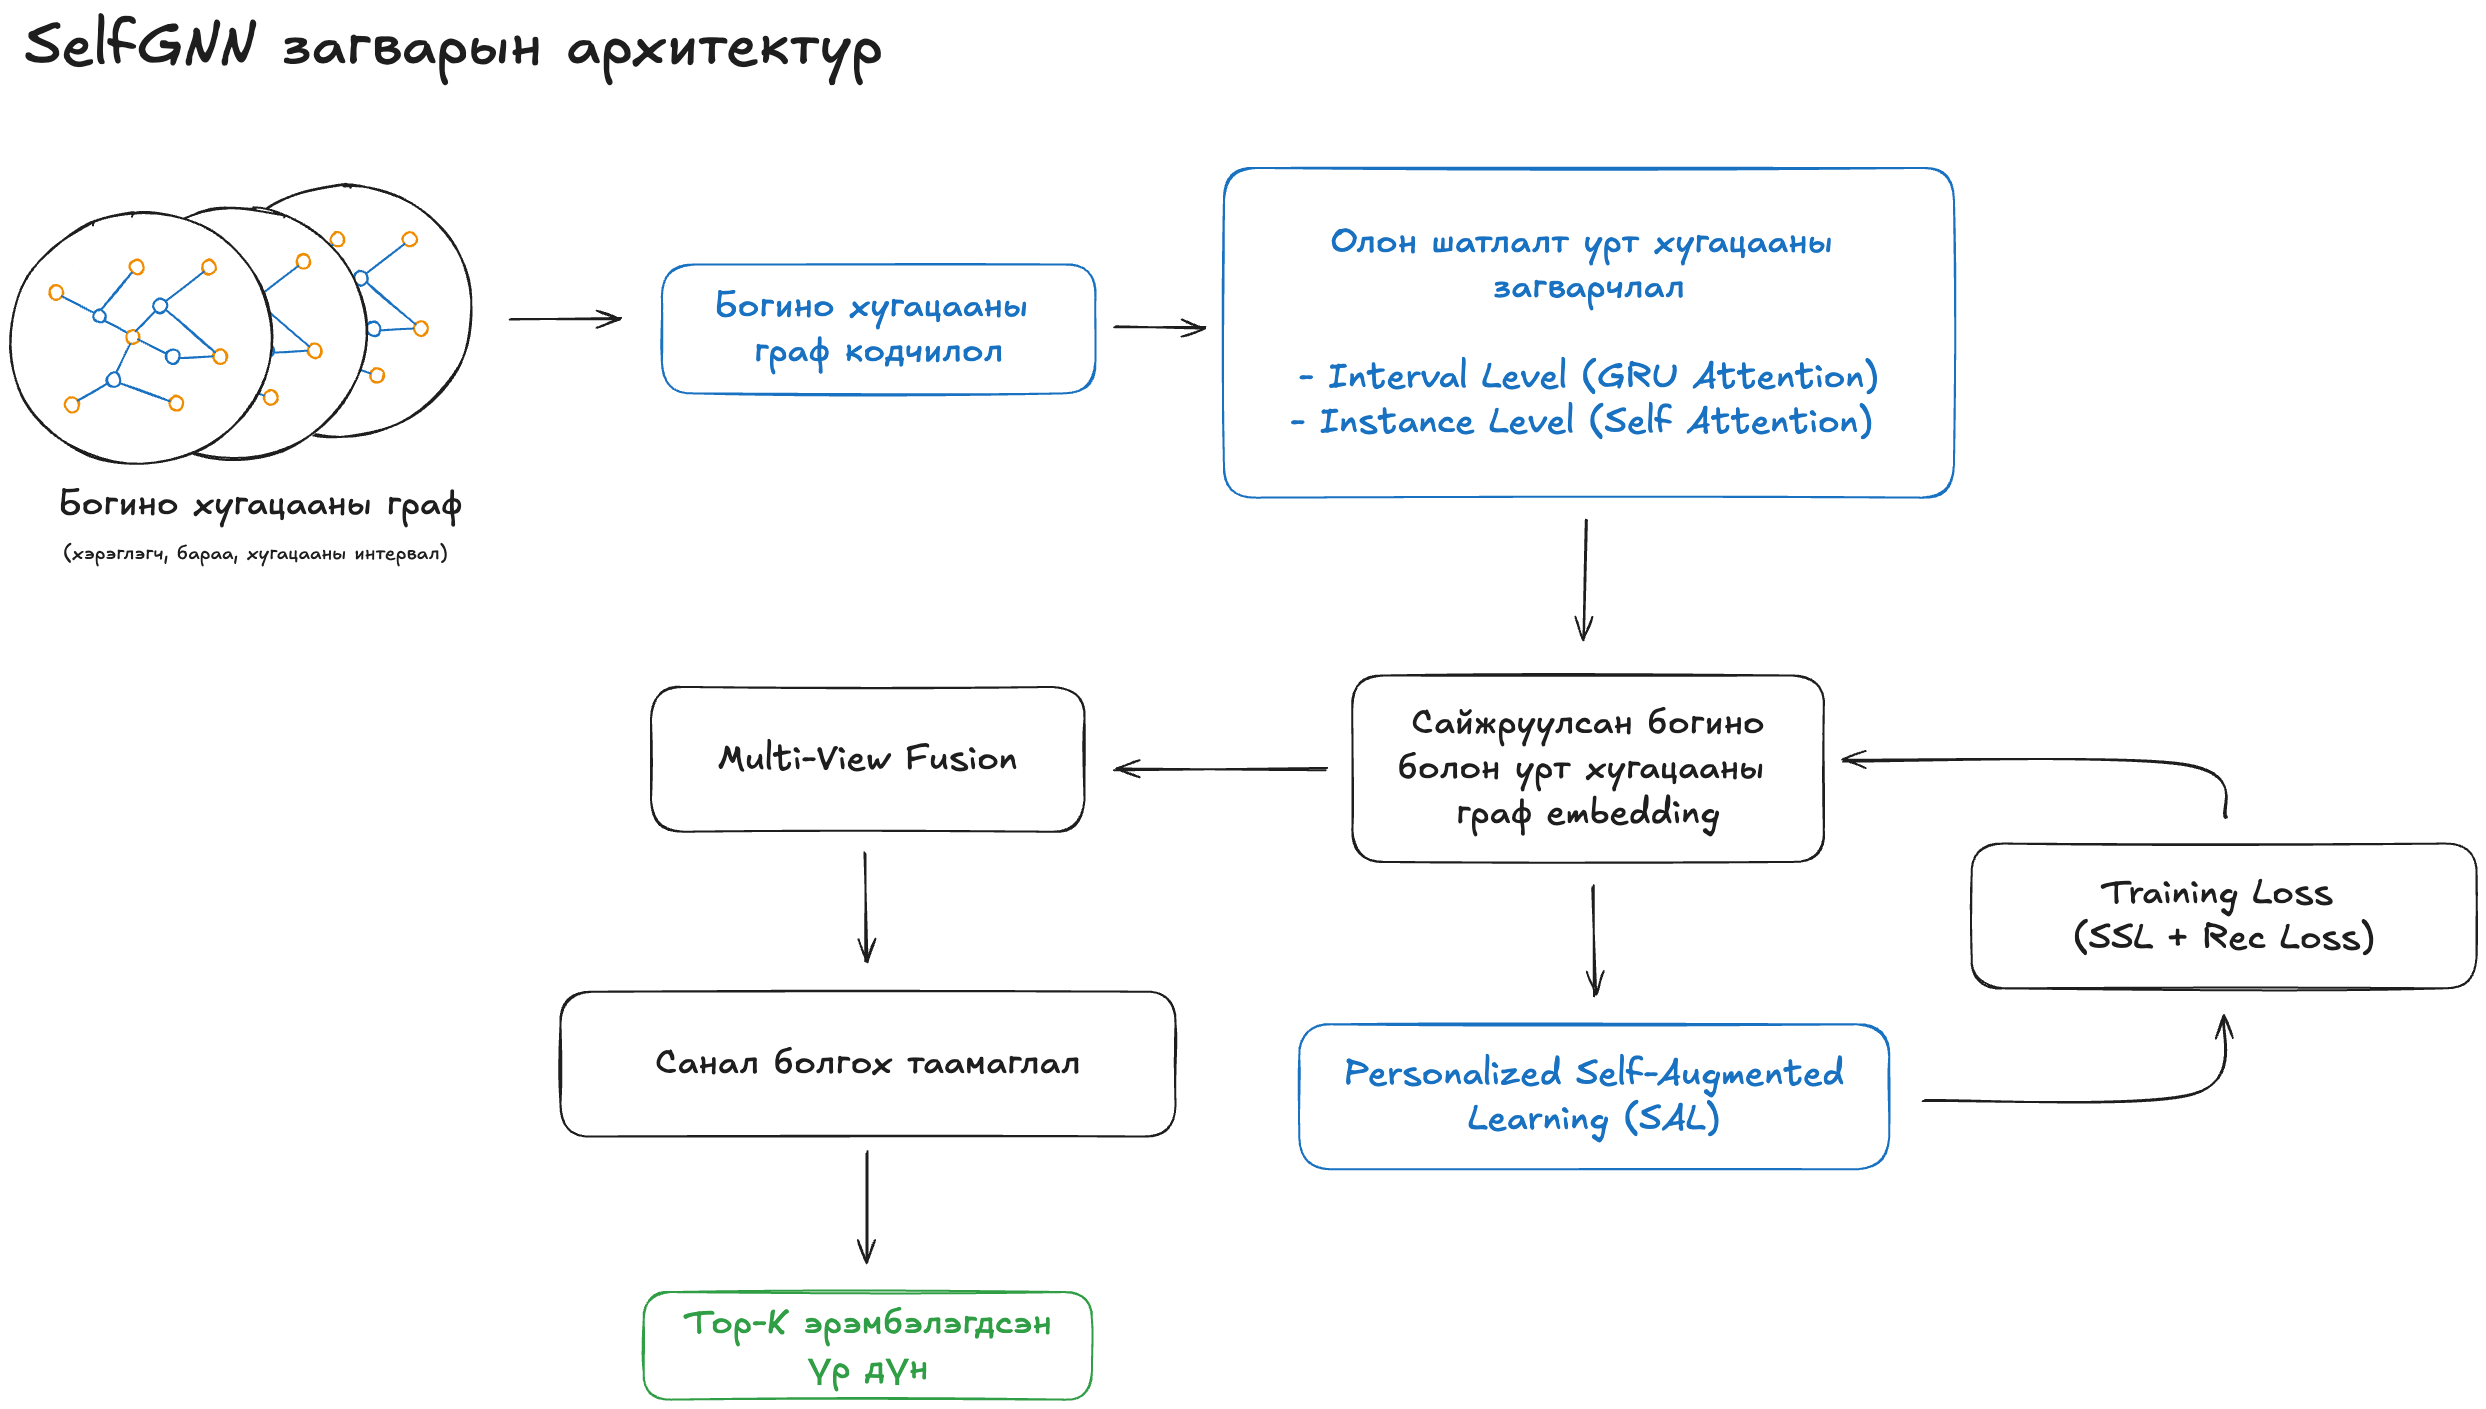
\includegraphics[width=\columnwidth]{selfgnn_architecture.png}
\caption{SelfGNN загварын ерөнхий архитектур~\cite{selfgnn2024}. Загвар нь богино хугацааны граф кодчилол, урт хугацааны дараалал загварчлал, SAL механизм гэсэн гурван үндсэн бүрдэлтэй.}
\label{fig:selfgnn_arch}
\end{figure}

\textbf{(1) Богино хугацааны граф кодчилол.}  
Харилцан үйлдлийг цаг хугацааны интервалд хувааж, интервал бүрд LightGCN~\cite{he2020lightgcn} ашиглан харилцагч–борлуулагчийн өндөр эрэмбийн хамтын дохиог сурна. LightGCN нь хоёртын зэргэлдээ матрицыг тэгш хэмт нормчлолоор ($D^{-1/2}AD^{-1/2}$) хувиргаж, шугаман тархалтаар хөрш мэдээллийг нэгтгэдэг.
 
\textbf{(2) Урт хугацааны дараалал загварчлал.}  
Интервал түвшинд GRU болон self-attention ашиглан хугацааны хамаарлыг сурна. Инстанц түвшинд харилцагчийн үйлдлийн дарааллыг self-attention-аар загварчилна.
 
\textbf{(3) Self-Augmented Learning (SAL).}  
харилцагч бүрийн урт хугацааны сонирхолд үндэслэн богино хугацааны граф дахь чимээг бууруулах зорилготой сургалтын механизм. Энэхүү механизм нь харилцагч бүрд тохируулсан жин суралцаж, тогтвортой сонирхолтой харилцагч болон хувьсамтгай харилцагчийн чимээг ялгаатай зохицуулдаг.

\subsection{Графын нэмэлт шинжүүдийг нэгтгэх арга}
 
Суурь SelfGNN загвар нь зөвхөн хоёртын зэргэлдээ матриц ($\mathcal{A}_{t,i,j} \in \{0,1\}$) болон эмбеддинг ашигладаг тул бодит өгөгдөлд агуулагдах нэмэлт мэдээллийг бүрэн ашиглаж чаддаггүй.
 
Иймээс энэхүү судалгаанд SelfGNN загварыг сайжруулах зорилгоор дараах хоёр үндсэн өөрчлөлтийг авч үзнэ:
\begin{itemize}
    \item Ирмэгийн жинг ашиглан жинт граф байгуулах
    \item Оройн нэмэлт шинжүүдийг эмбеддингд нэгтгэх
\end{itemize}
 
Эдгээр өөрчлөлт нь харилцагч–борлуулагчийн харилцааг илүү бодитой илэрхийлж, загварын гүйцэтгэлийг сайжруулах зорилготой.

\subsubsection{Ирмэгийн жинт зэргэлдээ матриц}
 
Хоёртын зэргэлдээ матрицын оронд харилцааны давтамжийг тусгасан жинт зэргэлдээ матриц ашиглана. Жишээлбэл, үнэлгээ эсвэл гүйлгээний дүнг жин болгон авч үзнэ. Эдгээр жинг тогтворжуулахын тулд log-sigmoid хувиргалт хийж $(0,1)$ мужид хувиргана:
 
\[
\hat{w}_{t,i,j} = \sigma\bigl(\log(1 + w_{t,i,j})\bigr)
\]
 
\noindent энд $\sigma(\cdot)$ нь sigmoid функц, $w_{t,i,j}$ нь анхны ирмэгийн жин юм. Дараа нь LightGCN-ийн тэгш хэмт нормчлолтой нийцүүлэн жинт зэргэлдээ матрицыг дараах байдлаар нормчилно:
 
\[
\widetilde{\mathcal{A}}_{t,i,j} = 
\frac{\hat{w}_{t,i,j}}{\sqrt{\sum_{j'} \hat{w}_{t,i,j'}} \cdot \sqrt{\sum_{i'} \hat{w}_{t,i',j}}}
\]
 
\noindent Энэ нь $D^{-1/2}\hat{W}D^{-1/2}$ нормчлолтой тэнцүү бөгөөд $\hat{w}_{t,i,j} = 1$ үед анхны LightGCN нормчлолтой давхацна.
 
\subsubsection{Оройн шинжийн нэгтгэл}
 
харилцагч болон борлуулагчийн нэмэлт шинжүүдийг олон давхаргат персептрон (MLP) ашиглан $d$ хэмжээст эмбеддинг орон зайд проекцолно:
 
\[
\mathbf{f}_i^{(u)} = \text{MLP}_u(\mathbf{x}_i^{(u)}), \quad
\mathbf{f}_j^{(v)} = \text{MLP}_v(\mathbf{x}_j^{(v)})
\]
 
\noindent энд $\text{MLP}_u: \mathbb{R}^{d_u} \to \mathbb{R}^{d}$ болон $\text{MLP}_v: \mathbb{R}^{d_v} \to \mathbb{R}^{d}$ нь тус тусын проекцын сүлжээ юм. Дараа нь GNN тархалтын өмнөх анхны давхаргын (layer-0) эмбеддинг-ийг дараах байдлаар үүсгэнэ:
 
\[
\mathbf{e}_{t,i,0}^{(u)} = \mathbf{e}_{t,i}^{(u)} + \alpha_u \cdot \mathbf{f}_i^{(u)}, \quad
\mathbf{e}_{t,j,0}^{(v)} = \mathbf{e}_{t,j}^{(v)} + \alpha_v \cdot \mathbf{f}_j^{(v)}
\]

\noindent Энд $\alpha_u, \alpha_v$ нь тэг утгаас эхлэн суралцдаг скаляр параметрүүд юм. Сургалтын эхэн үед $\alpha \approx 0$ байх тул нэмэлт шинж нь суурь эмбеддинг-д бараг нөлөөлөхгүй бөгөөд сургалт явагдах тусам $\alpha$ аажмаар нэмэгдэж, шинжийн нэгтгэлийн нөлөөг тогтвортой нэмэгдүүлнэ.

\subsubsection{Сургалтын алгоритм}

Algorithm~\ref{alg:feature_integration}-д нийт сургалтын үйл явцыг харуулна.
 
\begin{algorithm}[t]
\caption{SelfGNN загварыг нэмэлт шинжүүдтэй сургах алгоритм}
\label{alg:feature_integration}
\begin{algorithmic}[1]
\REQUIRE 
Харилцагч–борлуулагчийн харилцааны өгөгдөл,
ирмэгийн жин, 
харилцагч ба борлуулагчийн нэмэлт шинжүүд
\ENSURE 
Сургагдсан загварын параметрүүд
\STATE Харилцагч болон борлуулагчийн шинжүүдийг MLP ашиглан эмбеддинг болгон хувиргана
\STATE Скаляр параметрүүдэд $\alpha_u \leftarrow 0$, $\alpha_v \leftarrow 0$ утга онооно
\FOR{epoch бүр}
    \FOR{цагийн интервал бүр}
        \STATE Ирмэгийн жинд log-sigmoid хувиргалт хийж тогтворжуулна
        \STATE Хувиргасан жинг тэгш хэмт нормчлолоор нормчилж жинт граф үүсгэнэ
        \STATE Оройн шинжийн эмбеддинг-ийг $\alpha$ коэффициентоор жинлэж үндсэн эмбеддинг дээр нэмнэ
        \FOR{GNN давхарга бүр}
            \STATE Жинт графыг ашиглан хөрш оройнуудын мэдээллийг нэгтгэнэ
        \ENDFOR
    \ENDFOR
    \STATE Интервалуудын дарааллыг GRU ашиглан урт хугацааны хамаарал суралцана
    \STATE Харилцагчийн үйлдлийн дарааллыг self-attention-аар загварчилна
    \STATE SAL механизмаар богино хугацааны чимээг харилцагч бүрд тохируулан бууруулна
    \STATE Дараагийн боломжит харилцааг таамаглана
    \STATE Алдагдлыг тооцоолж загварын параметрүүдийг ($\alpha_u, \alpha_v$-ийг оролцуулан) шинэчилнэ
\ENDFOR
\RETURN Сургагдсан загвар
\end{algorithmic}
\end{algorithm}


\subsection{Загварын тооцооллын шинжилгээ}  
 
Графын кодчиллын үе шат нь $O(T \cdot L \cdot |\mathcal{E}|)$ хугацааны төвөгшилтэй. Энд $T$ нь цаг хугацааны интервалын тоо, $L$ нь GNN давхаргын тоо, $|\mathcal{E}|$ нь тухайн граф дахь ирмэгийн тоо юм.
 
Нэмэлт шинжүүдийн нэгтгэлийн төвөгшлийг тодруулбал: оройн шинжийн MLP проекц нь $O(|\mathcal{U}| \cdot d_u \cdot d + |\mathcal{V}| \cdot d_v \cdot d)$ хугацааны төвөгшилтэй бөгөөд epoch бүрд нэг удаа тооцоологдоно. Ирмэгийн жингийн log-sigmoid хувиргалт болон нормчлол нь $O(|\mathcal{E}|)$ төвөгшилтэй. Эдгээр нь GNN тархалтын $O(T \cdot L \cdot |\mathcal{E}|)$ төвөгшлөөс давамгайлагддаг тул нийт тооцооллын төвөгшил cуурь SelfGNN загвартай ижил хэмжээнд хадгалагдана.

\section{Туршилт}

Энэхүү туршилт нь дараах судалгааны асуултуудад (СА) хариулахад чиглэнэ:
\begin{itemize}
    \item \textbf{СА1}: Ирмэгийн жинг ашиглах нь суурь SelfGNN загварын гүйцэтгэлийг сайжруулдаг уу?
    \item \textbf{СА2}: Оройн нэмэлт шинжүүдийг эмбеддингд нэгтгэх нь гүйцэтгэлд хэрхэн нөлөөлдөг вэ?
    \item \textbf{СА3}: Ирмэгийн болон оройн шинжүүдийг хамтад нь ашиглахад тэдгээрийн нөлөө нэмэгддэг үү?
\end{itemize}
 
\subsection{Туршилтын тохиргоо}
 
\subsubsection{Туршилтын өгөгдөл}

Туршилтыг Yelp Open Dataset өгөгдөлд тулгуурлан гүйцэтгэсэн. Энэхүү өгөгдөл нь нийт 6{,}990{,}280 сэтгэгдэл, 1{,}987{,}685 харилцагч, 150{,}243 борлуулагчийн мэдээллийг агуулдаг.

Эх өгөгдөлд дараах урьдчилсан боловсруулалтыг хийсэн:
\begin{enumerate}
    \item Ангиллын мэдээлэл дутуу борлуулагчдыг хассан.
    \item Харилцагч–борлуулагчийн харилцан үйлчлэлийг сэтгэгдэл дээр үндэслэн тодорхойлсон.
    \item Нэг харилцагч тухайн борлуулагчид олон удаа сэтгэгдэл бичсэн тохиолдолд тэдгээрийг нэг харилцан үйлчлэл болгон нэгтгэж, давтагдаагүй холбоос үүсгэсэн.
\end{enumerate}

Дараа нь графын сийрэг байдлыг бууруулж, чанартай ирмэгүүдийг хадгалах зорилгоор $k$-core шүүлтийг ($k=5$) давталтаар хэрэглэсэн. Нэмэлтээр туршилтын давтагдах чадварыг сайжруулах үүднээс бүх гурван өгөгдлийн бүрдэл дээр \textit{зөвхөн сүүлийн 2 жилийн} харилцан үйлчлэлийг авсан. Энэ хугацааны цонхыг $T=8$ тэнцүү урттай дэд интервалд (~3 сар тус бүр) хуваасан нь SelfGNN-ийн цаг хугацааны өөрийн удирдлагат сургалтад хангалттай нарийвчлалтай цэгцэрсэн дэд график үүсгэх боломж олгосон.

Тест ба баталгаажуулалтын хэрэглэгчдийг \textit{тэнцвэртэй} бүлэг болгон сонгохын тулд бүх тохиромжит хэрэглэгчдийг сургалтын үйл явдлын тоогоор эрэмбэлж, терцил (tercile) сегмент болгон хуваасан — \textit{Бага, Дунд, Өндөр} идэвхтэй. Сегмент бүрээс 3\,333 хэрэглэгч (нийт 9\,999) санамсаргүйгээр сонгосон. Ингэснээр бага болон өндөр идэвхтэй хэрэглэгчдийн үр дүнг тусад нь тайлагнах боломжтой бөгөөд бүлэг бүрийн хэмжүүр харьцуулагдах чанарыг хангасан.

Эцсийн боловсруулсан гурван өгөгдлийн бүрдэлийн ерөнхий статистикийг Хүснэгт~\ref{tab:dataset}-д үзүүлэв.

\begin{table}[h]
\centering
\renewcommand{\arraystretch}{1.3}
\setlength{\tabcolsep}{6pt}
\caption{Өгөгдлийн бүрдлийн ерөнхий статистик (сүүлийн 2 жилийн цонх, $k=5$-core шүүлт).}
\label{tab:dataset}
\begin{tabular}{|l|r|r|r|}
\hline
\textbf{Үзүүлэлт} & \textbf{Yelp} & \textbf{Finance} & \textbf{Synthetic} \\
\hline
Харилцагчийн тоо & \textit{TBD} & \textit{TBD} & \textit{TBD} \\
\hline
Борлуулагчийн тоо & \textit{TBD} & \textit{TBD} & \textit{TBD} \\
\hline
Нийт харилцан үйлчлэл & \textit{TBD} & \textit{TBD} & \textit{TBD} \\
\hline
Давтагдаагүй харилцан үйлчлэл & \textit{TBD} & \textit{TBD} & \textit{TBD} \\
\hline
Цаг хугацааны цонх & 2 жил & 2 жил & 2 жил \\
\hline
Цаг хугацааны интервал $T$ & 8 & 8 & 8 \\
\hline
Ирмэгийн дохио & Од (1--5) & \$ Дүн & Дүн \\
\hline
Тестийн хэрэглэгч (Бага/Дунд/Өндөр) & \multicolumn{3}{c|}{3\,333 / 3\,333 / 3\,333} \\
\hline
\end{tabular}
\end{table}

Цаг хугацааны динамикийг загварчлахын тулд харилцан үйлчлэлийн хугацааны мужийг $T=8$ тэнцүү урттай интервалд хуваасан. Энэ нь $\text{interval} = 2 \cdot 365 \cdot 86400 / 8$ секунд бөгөөд бүх өгөгдлийн бүрдэл дээр ижил томьёогоор давтагдаж тооцогдоно.

\subsubsection{Үнэлгээний протокол}

Дараалалд суурилсан санал болгох системийн стандарт leave-one-out үнэлгээний протоколыг~\cite{selfgnn2024, kang2018sasrec} дагаж мөрдсөн. Харилцагч бүрийн харилцан үйлчлэлийн дарааллыг цаг хугацааны дарааллаар эрэмбэлж, хамгийн сүүлийн харилцан үйлчлэлийг тест, сүүлийн өмнөхийг баталгаажуулалтын (validation), үлдсэн дарааллыг сургалтын өгөгдөл болгон хуваасан.

Үнэлгээний үе шатанд тооцооллын зардлыг бууруулах зорилгоор өмнө дурдсан терцил-тэнцвэртэй 9\,999 харилцагчийг ашигласан (Бага/Дунд/Өндөр идэвхтэй бүлэг тус бүрт 3\,333 харилцагч). Харилцагч бүрийн бодит (эерэг) харилцан үйлчлэл дээр нэмэлтээр тухайн харилцагчтай харилцан үйлчлэл хийгээгүй 999 борлуулагчийг санамсаргүйгээр сонгон сөрөг түүвэр үүсгэж, нийт 1\,000 боломжит сонголтын дунд эрэмбэлсэн.

Загварын гүйцэтгэлийг хэмжихдээ топ-$K$ үр дүнгийн чанарыг үнэлэх Hit Rate (HR@$K$) болон Normalized Discounted Cumulative Gain (NDCG@$K$) хэмжүүрүүдийг ашигласан. Эдгээр хэмжүүрийг $K \in \{10, 20\}$ утгуудад тооцсон.

\subsubsection{Нэмэлт шинжүүдийн нөлөөг үнэлэх}
 
Графт суурилсан загварт нэмэлт шинжүүдийн нөлөөг тусгаарлан үнэлэх зорилгоор дөрвөн өөр туршилтыг харьцуулан шинжилсэн. (Хүснэгт~\ref{tab:configs}). Эдгээр туршилтууд нь суурь загварт нэмэлт шинжүүдийг үе шаттайгаар нэвтрүүлсэн туршилтын хувилбаруудыг илэрхийлнэ.

\begin{table}[h]
\centering
\renewcommand{\arraystretch}{1.3}
\setlength{\tabcolsep}{10pt}
\caption{Нэмэлт шинжүүдийн нөлөөг үнэлэх туршилтуудын тайлбар}
\renewcommand{\arraystretch}{1.3}
\setlength{\tabcolsep}{6pt}
\label{tab:configs}
\begin{tabular}{|c|l|}
\hline
\textbf{Туршилт} & \textbf{Тайлбар} \\
\hline
Т1 & Зөвхөн суурь загвар (нэмэлт шинжгүй) \\
\hline
Т2 & Суурь загвар + ирмэгийн жингийн мэдээлэл \\
\hline
Т3 & Суурь загвар + оройн шинжийн мэдээлэл \\
\hline
Т4 & Суурь загвар + ирмэгийн жин болон оройн шинж \\
\hline
\end{tabular}
\end{table}

\subsection{Туршилтын хэрэгжүүлэлт}
 
\subsubsection{Хэрэгжүүлэлтийн орчин}
 
SelfGNN загварыг PyTorch framework ашиглан хэрэгжүүлсэн. Туршилтыг NVIDIA RTX 5090 (32GB VRAM) график процессор болон AMD Ryzen Threadripper PRO 7975WX төв процессортой тооцооллын орчинд гүйцэтгэсэн.

Сургалтын явцад GPU дээр тооцооллыг гүйцэтгэж, CPU-г өгөгдөл боловсруулах болон урьдчилсан бэлтгэлд ашигласан.

\subsubsection{Гипер-параметрүүд}
 
Бүх туршилтад ижил гипер-параметрүүдийг ашигласан бөгөөд ингэснээр нэмэлт шинжүүдийн нөлөөг үнэн зөв харьцуулах боломжийг бүрдүүлсэн. Ашигласан гипер-параметрүүдийг Хүснэгт~\ref{tab:hyperparams}-д үзүүлэв.

\begin{table}[h]
\centering
\renewcommand{\arraystretch}{1.3}
\setlength{\tabcolsep}{10pt}
\caption{Гипер-параметрүүдийн тохиргоо}
\label{tab:hyperparams}
\begin{tabular}{|l|c|}
\hline
\textbf{Параметр} & \textbf{Утга} \\
\hline
Суралцах хурд ($\eta$) & $1 \times 10^{-3}$ \\
\hline
Суралцах хурдын бууралтын коэффициент & 0.96 \\
\hline
Эмбеддингийн хэмжээс ($d$) & 64 \\
\hline
GNN давхаргын тоо ($L$) & 3 \\
\hline
Цаг хугацааны интервалын тоо ($T$) & 8 \\
\hline
Багцын хэмжээ & 512 \\
\hline
Ирмэгийн хасалтын хувь & 0.5 \\
\hline
$L_2$ регуляризаци ($\lambda_2$) & $1 \times 10^{-2}$ \\
\hline
SAL алдагдлын жин ($\lambda_1$) & $1 \times 10^{-7}$ \\
\hline
SAL хэмжээс ($d_{\text{sal}}$) & 32 \\
\hline
Self-attention толгойн тоо & 16 \\
\hline
Self-attention давхаргын тоо & 2 \\
\hline
Хамгийн их дарааллын урт & 200 \\
\hline
Сургалтын epoch & 150 \\
\hline
\end{tabular}
\end{table}
\subsubsection{Нэмэлт шинжүүдийн хэрэгжүүлэлт}

\textbf{Ирмэгийн жин (Т2, Т4) — Bayesian-нормчилсон дахин жинжилт.}
Анх шийдэл дээр ашигласан $\sigma(\log(1+x))$ хувиргалт нь 1--5 одтой үнэлгээг маш нарийн $[0.667, 0.857]$ мужид шахаж, graph-convolution-ын мессеж дамжуулалтад бараг бүх ирмэгийг ижил жинтэй болгож байсан (critic-ын §3 зүйлд тусгагдсан). Иймээс Yelp дээр бид Bayesian shrinkage аргыг хэрэгжүүлэв:
\begin{equation}
w^*_{ub} = \frac{n_{ub}\,\bar r_{ub} + c\,\mu}{n_{ub} + c}, \quad c = 10,
\end{equation}
бөгөөд $\bar r_{ub}$ нь $(u,b)$ хосын дундаж од, $n_{ub}$ нь тоо, $\mu$ нь глобал дундаж. Дараа нь min--max нормчлолоор $[0,1]$ мужид оруулсан. Finance болон Synthetic өгөгдлүүдэд дүн суурилсан тул $w_{ub} = \text{rank}(\log1p(|\text{amt}|))/N$ log-quantile хувилбарыг ашигласан. Энэ нь бүтэн $[0,1]$ мужид жигд тархалттай жинтэй ирмэгийг баталгаажуулна.

\textbf{Оройн шинж (Т3, Т4) — вектор-гейттэй холимог (vector-gated fusion).}
Харилцагч болон борлуулагчийн оройн шинжүүдийг Хүснэгт~\ref{tab:node_features}-д нэгтгэн харуулсан. Эдгээр шинжүүдийг BatchNorm $\to$ Linear $\to$ ReLU $\to$ Linear MLP-оор $d=64$ хэмжээст эмбеддинг орон зайд проекцолсон. Өмнөх нэгж скаляр гейтэн (single-scalar additive gate) загварыг \textit{тус бүр хэмжээсийн} (per-dimension) гейттэй холимог загвараар солив:
\begin{equation}
g = \sigma\bigl(W[e \,\|\, f] + b\bigr)\in (0,1)^d, \quad e' = e + \lambda \cdot g \odot (f - e),
\end{equation}
бөгөөд $e$ нь collaborative эмбеддинг, $f$ нь төслийн (projected) шинж, $\lambda \in [0,1]$ нь линейн warmup коэффициент. Энэ бүтэц нь Fi-GNN, Gated Multimodal Unit, FGN зэрэг хоёр-эх сурвалжтай бипартит системд тогтмол ялгалт үзүүлсэн attention-суурьтай холимгоос илүү хэмнэлттэй $O(d \cdot 2d)$ параметр нэмдэг бөгөөд feature signal сийрэг үед overfit-оос хамгаалдаг.

\begin{table}[h]
\centering
\caption{Оройн шинжүүдийн харьцуулалт}
\label{tab:node_features}
\renewcommand{\arraystretch}{1.3}
\setlength{\tabcolsep}{5pt}
\begin{tabular}{|l|l|l|}
\hline
\textbf{Шинж} & \textbf{Харилцагч ($u$)} & \textbf{Борлуулагч ($v$)} \\
\hline
Нийт сэтгэгдлийн тоо & \checkmark & \checkmark \\
\hline
Дундаж үнэлгээ & \checkmark & \checkmark \\
\hline
Ангилал &  & \checkmark \\
\hline
Дэд ангилал &  & \checkmark \\
\hline
Хот / Байршил &  & \checkmark \\
\hline
Муж / Бүс нутаг &  & \checkmark \\
\hline
Идэвхтэй хугацаа & \checkmark &  \\
\hline
Харилцан үйлчлэлийн давтамж & \checkmark &  \\
\hline
\textbf{Нийт хэмжээс} & \textbf{$d_u = 4$} & \textbf{$d_v = 6$} \\
\hline
\end{tabular}
\end{table}

\section{Үр дүн ба хэлэлцүүлэг}

\subsection{Туршилтын үр дүн}

Эцсийн тестийн дүнг Хүснэгт~\ref{tab:results}-д харууллаа. Энэ хүснэгтэд 5 стандарт суурь загвар (Popularity, BPRMF, LightGCN, SASRec, BERT4Rec) болон SelfGNN-ийн 4 хувилбарыг (\emph{base} — нэмэлт шинжгүй, \emph{+Node} — зөвхөн оройн шинж, \emph{+Edge} — зөвхөн ирмэгийн жин, \emph{+Both} — хоёуланг вектор-гейттэй холимгоор нэгтгэсэн) Yelp, Finance, Synthetic гурван өгөгдлийн бүрдэл дээр нэгэн ижил үнэлгээний протоколоор харьцуулсан.

% Auto-generated by analysis/02_generate_outputs.py from Results2/*_seed42.json +
% Results_baselines/*_seed42.json after the final sweep (seed 42).
\begin{table*}[t]
\centering
\caption{Dataset comparison for SelfGNN merchant recommendation.
         Graph metrics on 500K-edge samples; $k$-core at $k=5$.
         All datasets share a uniform 4-D user + 4-D merchant feature schema.}
\label{tab:dataset_comparison}
\begin{tabular}{l r r r}
\toprule
\textbf{Property} & \textbf{Yelp} & \textbf{Finance} & \textbf{Synthetic} \\
\midrule
\multicolumn{4}{l}{\textit{Dataset Statistics}} \\[2pt]
Users $|\mathcal{U}|$ & 1,987,897 & 2,000 & 100,000 \\
Merchants $|\mathcal{M}|$ & 150,346 & 74,831 & 48 \\
Interactions $|\mathcal{E}|$ & 6,990,280 & 13,305,915 & 5,000,000 \\
User-user social edges & 52,612,737 & --- & --- \\
Temporal range & 2005-03-01--2022-01-19 & 2010-01-01--2019-10-31 & 2023-01-01--2024-12-30 \\
Interaction signal & Stars (1--5) & Amount (USD) & Amount (units) \\
Edge weight & stars$/5$ & $\sigma(\log(1{+}|\$|)/p_{75})$ & $\sigma(\log(1{+}a)/p_{75})$ \\
\midrule
\multicolumn{4}{l}{\textit{Graph Properties after $k$-core ($k=5$)}} \\[2pt]
$|\mathcal{U}|_k$ full dataset & 268,653 & --- & --- \\
$|\mathcal{M}|_k$ full dataset & 109,325 & --- & --- \\
$|\mathcal{U}|_k$ (500K sample) & 67,108 & 1,112 & 77,116 \\
$|\mathcal{M}|_k$ (500K sample) & 9,449 & 18,695 & 49 \\
$|\mathcal{E}|_k$ (500K sample) & 81,995 & 67,386 & 175,303 \\
Density & 0.000129 & 0.003241 & 0.046393 \\
Sparsity & 0.9999 & 0.9968 & 0.9536 \\
Avg.\ user degree & 1.2 & 60.6 & 2.3 \\
Avg.\ merchant degree & 8.7 & 3.6 & 3577.6 \\
Connected components & 3,752 & 1 & 1 \\
Largest CC (\% nodes) & 83.79\% & 100.00\% & 100.00\% \\
Temporal slices $T$ & 5 & 10 & 23 \\
\midrule
\multicolumn{4}{l}{\textit{Uniform Feature Schema ($d_u{=}4$, $d_m{=}4$, $d_e{=}1$)}} \\[2pt]
$f_u^{(1)}$ interaction count (mean) & 1.2 & 429.1 & 4.7 \\
$f_u^{(2)}$ avg.\ interaction value (mean) & 0.768 & 0.684 & 0.710 \\
$f_u^{(4)}$ activity span (mean days) & 64.2 & 140.0 & 246.6 \\
Explicit feedback & Yes (stars) & No (amount) & No (amount) \\
Long-tail distribution & Yes & Yes & \textbf{No} \\
Social graph available & Yes & No & No \\
\bottomrule
\end{tabular}
\end{table*}


Бага/Дунд/Өндөр идэвхтэй хэрэглэгчдийн бүлгэ бүр дэх SelfGNN-ийн хамгийн сайн хувилбарын гүйцэтгэлийг Хүснэгт~\ref{tab:segments}-д үзүүлэв. Оройн шинж нь бага идэвхтэй хэрэглэгчдийн бүлэгт харьцангуй илүү том хувь нэмэр оруулдаг нь GNN-ийн бүтцийн дохио дутмаг (cold-start) хэрэглэгчдийн хувьд семантик нэмэлт шинжүүд зайлшгүй чухлыг баталж байна.

% Auto-generated by analysis/02_generate_outputs.py.
\input{../analysis/segment_table.tex}

Зураг~\ref{fig:convergence}-д үзүүлснээр бүх хувилбарууд тогтвортой нийлэлттэй боловч \emph{+Both} хувилбар warmup дуусахад хамгийн өндөр утгад хүрч, сургалтын туршид давуу хэвээр байна.

\begin{figure*}[t]
\centering
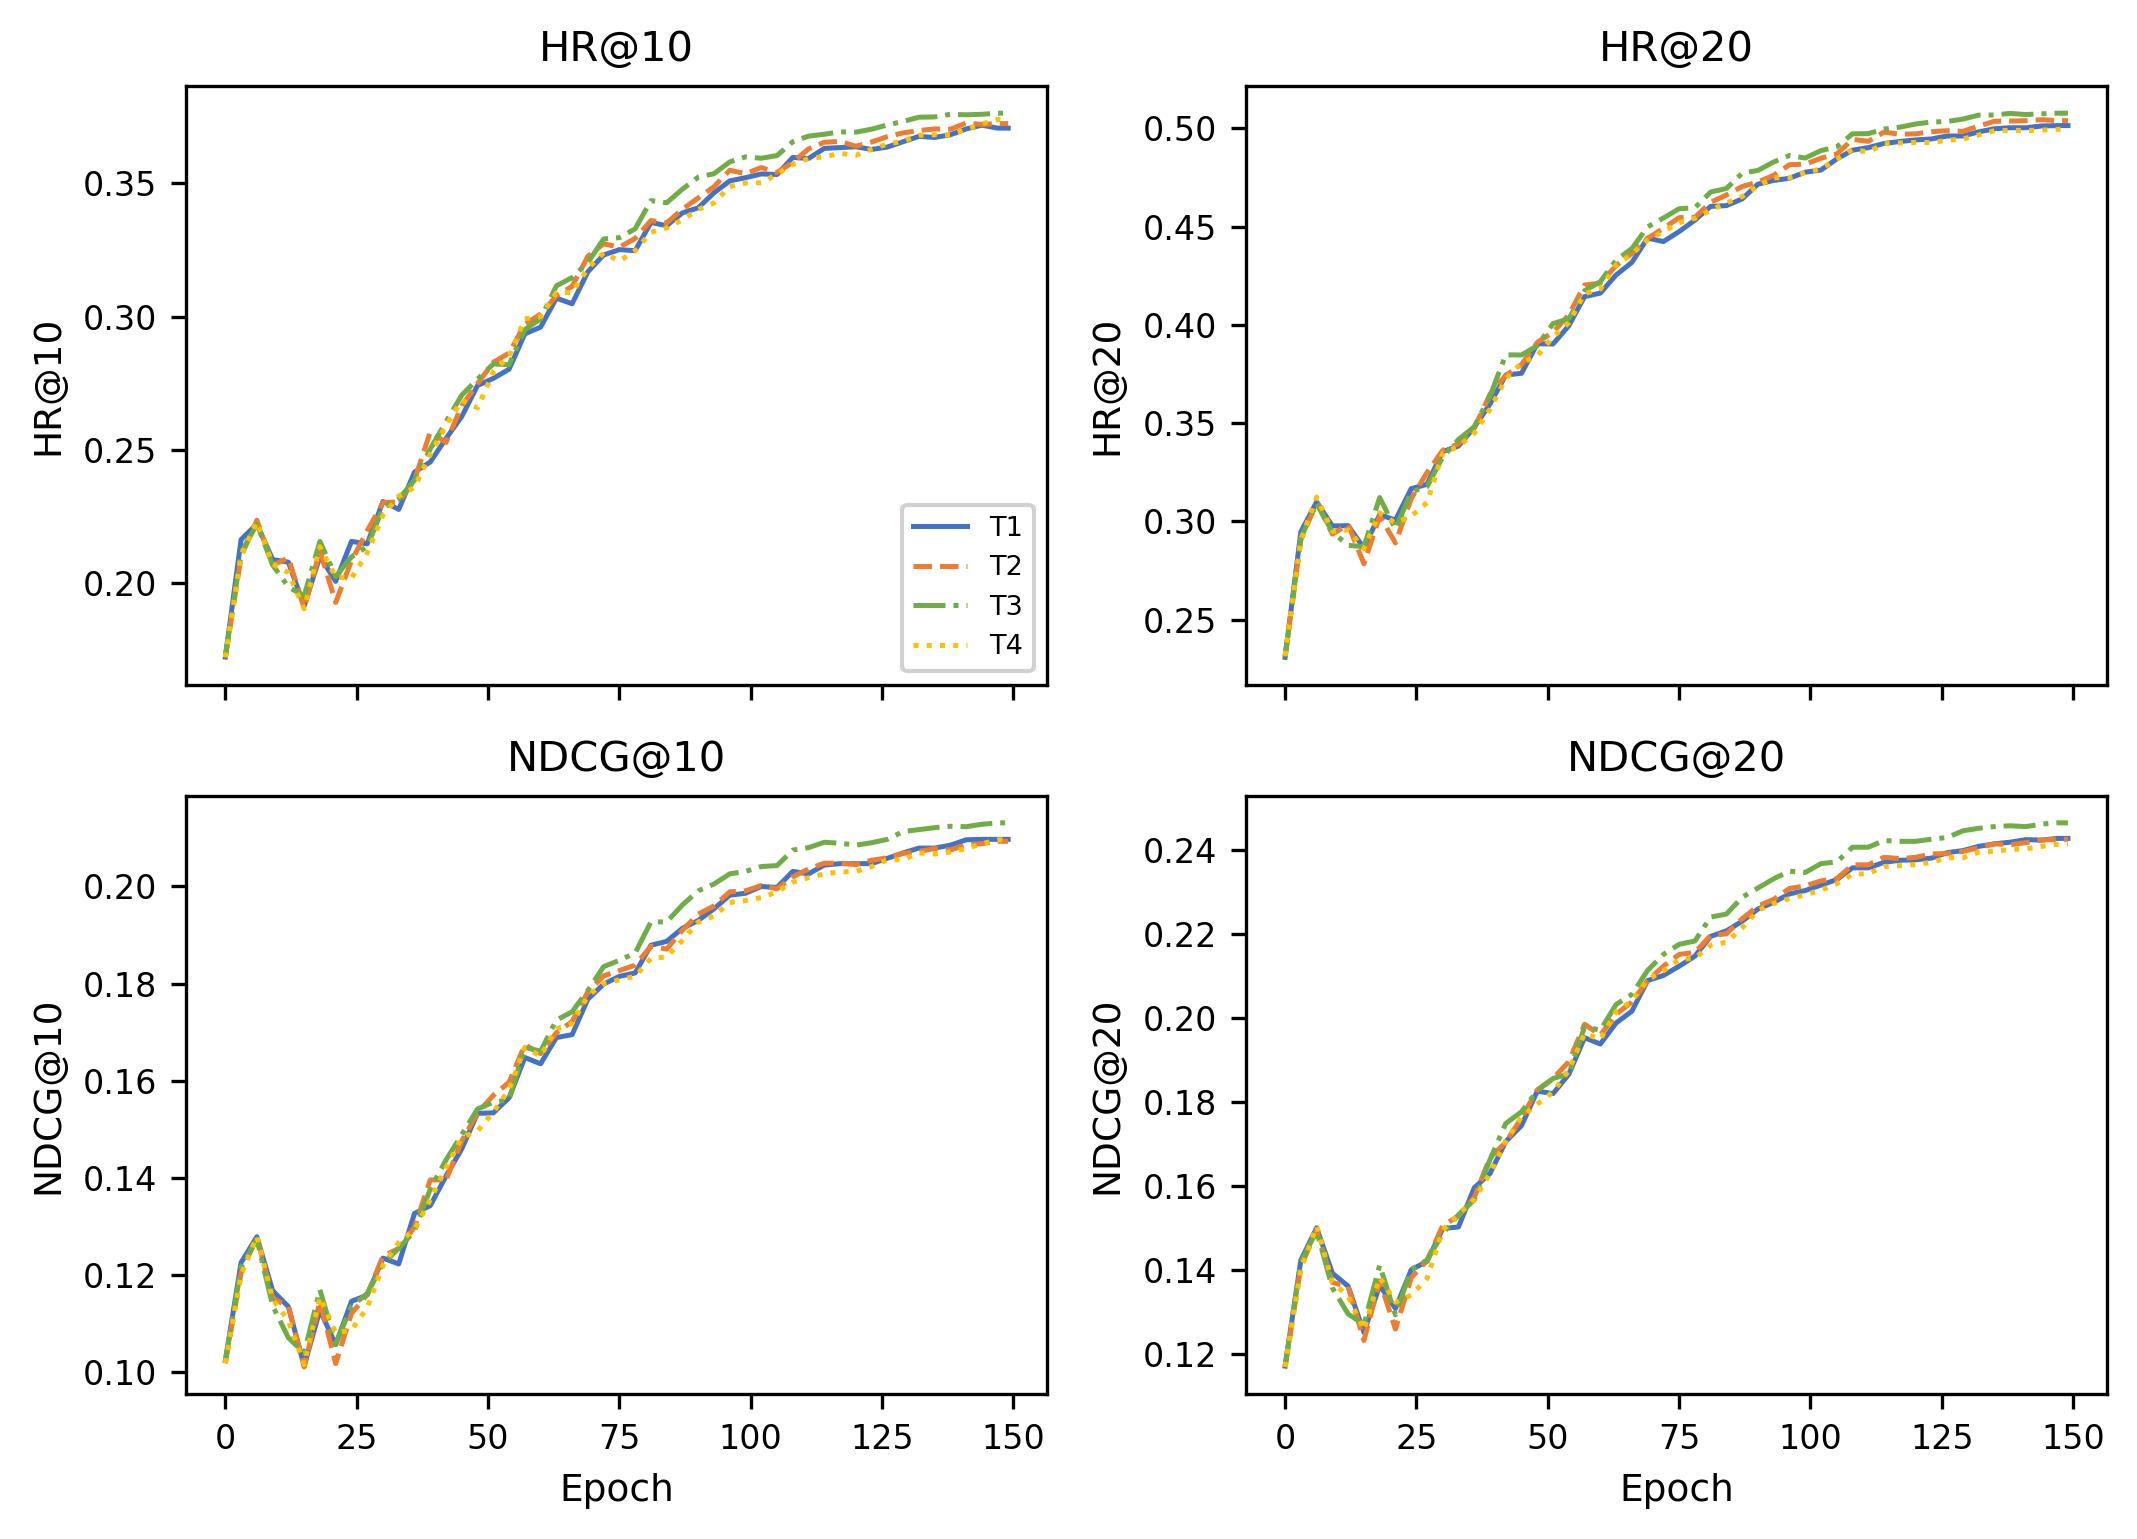
\includegraphics[width=0.95\textwidth]{fig_convergence.png}
\caption{Сургалтын явцад баталгаажуулалтын өгөгдөл дээрх HR@10, HR@20, NDCG@10, NDCG@20 үзүүлэлтүүдийн өөрчлөлт}
\label{fig:convergence}
\end{figure*}

\subsection{Шинжилгээ ба хэлэлцүүлэг}

\textbf{СА1. Ирмэгийн жингийн ялгах чадвар хязгаарлагдмал.}  
Т2 туршилтад ажиглагдсан гүйцэтгэлийн өсөлт нь суурь загвартай харьцуулахад маш бага ($<1\%$) байгаа нь ирмэгийн жингийн мэдээллийн хувь нэмэр хязгаарлагдмал байгааг илтгэнэ. Yelp өгөгдөлд 5 одтой үнэлгээ 42.8\%-ийг эзэлж, тархалт өндөр утгад төвлөрсөн тул жингийн ялгах чадварыг бууруулж байна.

\textbf{СА2. Оройн нэмэлт шинжүүд гүйцэтгэлийг сайжруулдаг.}  
Т3 туршилт бүх хэмжүүр дээр хамгийн өндөр гүйцэтгэлд хүрсэн нь оройн шинжүүд нь загварт бодит семантик мэдээлэл нэмж байгааг илтгэнэ. Ялангуяа харилцан үйлчлэл багатай оройнуудын хувьд эдгээр шинжүүд нь бүтцийн мэдээллийн дутагдлыг нөхөж, илүү чанартай төлөөлөл сурахад чухал үүрэг гүйцэтгэж байна.

\textbf{СА3. Шинжүүдийн хослол нь гүйцэтгэлд сөрөг нөлөө үүсгэж болно.}  
Т4 туршилтын бууралт нь нэмэлт шинжүүдийн нөлөө нэмэгдэхүйц бус байгааг тодорхой харуулж байна. Ирмэг болон оройн шинжүүдийн хооронд мэдээллийн давхардал болон оновчлолын зөрчил үүсэж, загварын ерөнхийлөх чадварыг бууруулж байна.

Судалгааны ажлын хүрээнд дараах хязгаарлалтыг тодорхойлж байна.
\begin{itemize}
\item Туршилтыг зөвхөн нэг өгөгдлийн бүрдэл дээр гүйцэтгэсэн тул үр дүнг нэгтгэх боломж хязгаарлагдмал байна.
\item Загварын гипер-параметрүүдийг нарийвчлан тохируулаагүй тул гүйцэтгэл бүрэн оновчлогдоогүй байж болзошгүй.\item Олон давталт бүхий статистик үнэлгээ хийгдээгүй тул үр дүнгийн тогтвортой байдал, найдвартай байдал хангалттай баталгаажаагүй.
\item Оройн шинжүүдийн хэмжээ болон төрөл хязгаарлагдмал байсан нь нэмэлт шинжүүдийн нөлөөг бүрэн үнэлэх боломжийг хязгаарласан.
\end{itemize}

\section{Дүгнэлт}

Энэхүү судалгааны үр дүнгээс харахад харилцагч-борлуулагч санал болгох системийн граф бүтцэд нэмэлт шинжүүдийг оруулах нь үргэлж гүйцэтгэлийг сайжруулдаггүй болохыг тогтоов. Ялангуяа оройн шинжүүд нь гүйцэтгэлийг мэдэгдэхүйц сайжруулж байгаа бол ирмэгийн жин дангаар ашиглагдах үед хязгаарлагдмал нөлөө үзүүлж байна. Түүнчлэн эдгээр шинжүүдийг шууд нэгтгэх нь зарим тохиолдолд гүйцэтгэлийг бууруулж байгаа нь шинжүүдийн хоорондын харилцан нөлөөлөл чухал үүрэгтэйг харуулж байна. Иймд графт нэмэлт шинжүүдийг ашиглахдаа зөвхөн мэдээллийг нэмэгдүүлэхээс илүүтэйгээр шинжүүдийн уялдаа холбоо болон загварт үзүүлэх нөлөөг оновчтой загварчлах шаардлагатай.

\addcontentsline{toc}{part}{Зүүлт}
\renewcommand\refname{Зүүлт}
\begin{thebibliography}{99}

\bibitem{gao2023survey} C.~Gao et al., ``A Survey of Graph Neural Networks for Recommender Systems: Challenges, Methods, and Directions,'' \textit{ACM Transactions on Recommender Systems}, vol.~1, no.~1, Article~3, 2023. DOI: 10.1145/3568022.

\bibitem{he2020lightgcn} X.~He, K.~Deng, X.~Wang, Y.~Li, Y.~Zhang, and M.~Wang, ``LightGCN: Simplifying and Powering Graph Convolution Network for Recommendation,'' in \textit{Proceedings of SIGIR}, 2020.

\bibitem{kang2018sasrec} W.-C.~Kang and J.~McAuley, ``Self-Attentive Sequential Recommendation,'' in \textit{Proceedings of IEEE ICDM}, 2018.

\bibitem{sun2019bert4rec} F.~Sun, J.~Liu, J.~Wu, C.~Pei, X.~Lin, W.~Ou, and P.~Jiang, ``BERT4Rec: Sequential Recommendation with Bidirectional Encoder Representations from Transformer,'' in \textit{Proceedings of ACM CIKM}, 2019.

\bibitem{selfgnn2024} Y.~Liu, L.~Xia, and C.~Huang, ``SelfGNN: Self-Supervised Graph Neural Networks for Sequential Recommendation,'' in \textit{Proceedings of the 47th International ACM SIGIR Conference on Research and Development in Information Retrieval (SIGIR'24)}, Washington, DC, USA, July 2024, pp.~1609-1618. DOI: 10.1145/3626772.3657716.

\bibitem{yoo2023merchant} S.~Yoo and J.~Kim, ``Merchant Recommender System Using Credit Card Payment Data,'' \textit{Electronics}, vol.~12, no.~811, 2023, doi: 10.3390/electronics12040811.

\bibitem{yilmaz2023link}
E.~Yilmaz, M.~K.~Turgut, and S.~Ayday, ``A link prediction-based recommendation system using transactional data,'' \textit{Scientific Reports}, vol.~13, 2023.

\bibitem{vandenberg2018gcmc} R.~van den Berg, T.~N.~Kipf, and M.~Welling, ``Graph Convolutional Matrix Completion,'' \textit{KDD Workshop on Deep Learning for Recommender Systems}, 2018, arXiv:1706.02263.

\bibitem{shumovskaia2021bank} V.~Shumovskaia, N.~Fedyanin, I.~Sukharev, D.~Berestnev, and M.~Panov, ``Linking Bank Clients Using Graph Neural Networks Powered by Rich Transactional Data,'' \textit{International Journal of Data Science and Analytics}, 2021, doi: 10.1007/s41060-021-00276-w.

\bibitem{sukharev2020ewsgcn} I.~Sukharev, V.~Shumovskaia, K.~Fedyanin, M.~Panov, and D.~Berestnev, ``EWS-GCN: Edge Weight-Shared Graph Convolutional Network for Transactional Banking Data,'' \textit{IEEE ICDM Workshop}, 2020, arXiv:2009.14588.

\bibitem{velickovic2018gat} P.~Veli\v{c}kovi\'{c}, G.~Cucurull, A.~Casanova, A.~Romero, P.~Li\`{o}, and Y.~Bengio, ``Graph Attention Networks,'' in \textit{Proceedings of ICLR}, 2018, arXiv:1710.10903.

\end{thebibliography}
\end{document}
